\documentclass{beamer}				% Style for presenation (with transitions)
%\documentclass[trans]{beamer}			% Turn off all transitions (pauses)
%\documentclass[handout]{beamer}		% Handouts print

% For handouts print
\usepackage{pgfpages}
\mode<handout>{
	\usetheme{default}
	\setbeamercolor{background canvas}{bg=black!5}
	\pgfpagesuselayout{4 on 1}[letterpaper,landscape,border shrink=2.5mm]
}

\beamertemplatenavigationsymbolsempty % Turn off navigation icons and links

\usepackage[utf8]{inputenc}

%\usetheme{AnnArbor}
\usetheme{Warsaw}
\usecolortheme{wolverine}
\usefonttheme{serif}
\usepackage{lscape}
\usepackage{graphicx}
\usepackage{multirow}
\usepackage{wrapfig}

\setbeamersize{text margin left=1em,text margin right=1em}
\setbeamertemplate{itemize items}[circle]

% Header and footer colors
% (less distraction by gray color)
\setbeamercolor{section in head/foot}{fg=white,bg=gray!40!black}
\setbeamercolor{subsection in head/foot}{fg=black,bg=gray!30}

% Delare \mysectionpage as section intro page
\setbeamerfont{section title}{parent=title}
\setbeamercolor{section title}{parent=titlelike}
\defbeamertemplate*{my section page}{default}[1][]
{
	\centering
	\begin{beamercolorbox}[sep=8pt,center,rounded=true,shadow=true,#1]{section title}
		\usebeamerfont{section title}\insertsection\par
	\end{beamercolorbox}
	%\addtocounter{framenumber}{-1}
}
\newcommand*{\mysectionpage}{\usebeamertemplate*{my section page}}

\title{Comparison of Top trees implementations}
\subtitle{Master thesis defense}
\author{Jiří Setnička}
\institute[KAM]{Department of Applied Mathematics}
\date{6 June 2018}

\begin{document}

\def\O{{\cal O}}

\begin{frame}[plain]
\vfill
\begin{figure}
	\includegraphics[width=75mm,type=pdf,ext=.epdf,read=.epdf]{mff_logo_new-crop}
\end{figure}
\titlepage
\end{frame}

%%%%%%%%%%%%%%%%%%%%%%%%%%%%%%%%%%%%%%%%%%%%%%%%%%%%%%%%%%%%%%%%%%%%%%%%%%%%%%%%

\section{Introduction}
\subsection{Top Trees overview}

\begin{frame}{Top Trees overview}

Data structure (Alstrup, Holm, Lichtenberg and Thorup in 1997):
\begin{itemize}
	\item Build over dynamically updated underlying forest
	\item Top Trees = trees of {\bf clusters} (generalized edges)
	\item Quick path operations -- $\O(\log N)$
	\pause\item Multiple drivers (implementations)
\end{itemize}

\bigskip
\pause Works as {\bf blackbox} for users:
\begin{itemize}
	\item User defines functions for joining/splitting of clusters
	\item Structure is controlled by user methods -- {\bf Link, Cut and Expose}
\end{itemize}
\end{frame}


\begin{frame}{Clusters}

{\bf Cluster = generalized edge}
\begin{itemize}
\item Two endpoints
\item Represents some path
\end{itemize}

\bigskip\pause
Contraction of clusters:
\begin{itemize}
\item {\bf Compress}
	\begin{figure}[h]
	\centering
	\includegraphics[width=7cm]{chap01_compress.pdf}
	\end{figure}
\item {\bf Rake}
	\begin{figure}[h]
	\centering
	\includegraphics[width=7cm]{chap01_rake.pdf}
	\end{figure}
\end{itemize}

\end{frame}

\begin{frame}{Clusters -- example}
	\begin{figure}[h]
	\centering
	\includegraphics[width=11cm]{chap01_top_tree.pdf}
	\end{figure}
\end{frame}

\subsection{User interactions}
\begin{frame}{User functions}
User must provide functions:
\begin{itemize}
\item {\bf Create} -- initialize basic cluster from one underlying edge
\item {\bf Destroy} -- distribute information from basic cluster to the underlying edge
\item {\bf Join} -- combine two child clusters into one compress/rake cluster
\item {\bf Split} -- distribute information to children (opposite to Join)
\end{itemize}
\end{frame}

\begin{frame}{User methods}
User could operate the structure with:
\begin{itemize}
\item {\bf Join} -- join given vertices from different trees by the new edge
\item {\bf Cut} -- cut given edge
\item {\bf Expose} -- expose given path in the root cluster
\end{itemize}
\end{frame}

%%%%%%%%%%%%%%%%%%%%%%%%%%%%%%%%%%%%%%%%%%%%%%%%%%%%%%%%%%%%%%%%%%%%%%%%%%%%%%%%

\section{Implementations}
\begin{frame}
\mysectionpage
\end{frame}

\subsection{Self-Adjusting Top Trees}
\begin{frame}{Self-Adjusting Top Trees}

\begin{itemize}
\item {\it Self-Adjusting Top Trees} by Tarjan and Werneck in 2005
\pause
\item {\bf Amortized time} per operation: $\O(\log N)$
\bigskip\pause
\item {\bf Splaying} (changes inside one path -- compress clusters)\\ and {\bf
splicing} (change partitioning of the tree into paths)
	\smallskip
	\begin{figure}
	\centering
	\includegraphics[width=10cm]{chap05_splice2.pdf}
	\end{figure}
\end{itemize}

\end{frame}


\subsection{Topology trees}
\begin{frame}{Topology trees}

\begin{itemize}
\item {\it Maintaining Information in Fully-Dynamic Trees with Top Trees} by
Alstrup, Holm, Lichtenberg and Thorup in 2003
\bigskip\pause
\item Based on topology trees -- ternarization of vertices
\item {\bf Worst-case} time per operation: $\O(\log N)$
\item Expected larger multiplicative constant than the Self-Adjusting Top Trees implementation
\bigskip\pause
\item {\bf Different partitioning into clusters} -- Top clusters must be mapped onto topology clusters
\end{itemize}

\end{frame}

\begin{frame}{Topology trees -- mapping of clusters}
	\begin{figure}
	\centering
	\includegraphics[width=10cm]{chap06_tree_mapping.pdf}
	\end{figure}
\end{frame}

%%%%%%%%%%%%%%%%%%%%%%%%%%%%%%%%%%%%%%%%%%%%%%%%%%%%%%%%%%%%%%%%%%%%%%%%%%%%%%%%

\section{Experiments}
\begin{frame}
\mysectionpage
\end{frame}

\subsection{Maximum edge weight on path}
\begin{frame}{Maximum edge weight on path}

Updates on {\bf forest} -- operations:
\begin{itemize}
	\item Link, cut
	\item Add weight to all edges on given path
	\item Get maximum weight on given path
\end{itemize}

\bigskip\pause
User functions:
\begin{itemize}
\item Join -- maximum weight from children
\item Split -- lazy propagation of extra weight
\end{itemize}

\end{frame}

\subsection{Edge 2-connectivity}
\begin{frame}{Edge 2-connectivity}
By Holm, Lichtenberg and Thorup in {\it Poly-logarithmic
Deterministic Fully-dynamic Algorithms for Connectivity, Minimum Spanning Tree,
2-edge, and Biconnectivity (2011)}

\bigskip

Updates on {\bf generic graph} -- operations:
\begin{itemize}
	\item Link, cut
	\item Query if given vertices are edge 2-connected
\end{itemize}

\bigskip\pause
Details:
\begin{itemize}
\item Cover level of all edges (tree and non-tree)
\item Cover, Uncover and Recover operations -- {\bf multiple calls} to the
top trees methods -- $\O(\log^4 N)$ per operation
\pause\item Possibility to {\bf turn off expensive updates} during Expose\\ $\rightarrow$
query in $\O(\log N)$ instead of $\O(\log^3 N)$
\end{itemize}

\end{frame}

\subsection{Results}

\begin{frame}{Experiments strategy}
\begin{itemize}
\item Same sequence of operations for both implementations
\item Measured {\bf initialization time} and {\bf time per one operation}
\item Several runs for each input size -- computed mean and standard deviation
\end{itemize}
\end{frame}

\begin{frame}{Maximum edge weight on path}
	\vskip -3mm
	\begin{figure}
	\centering
	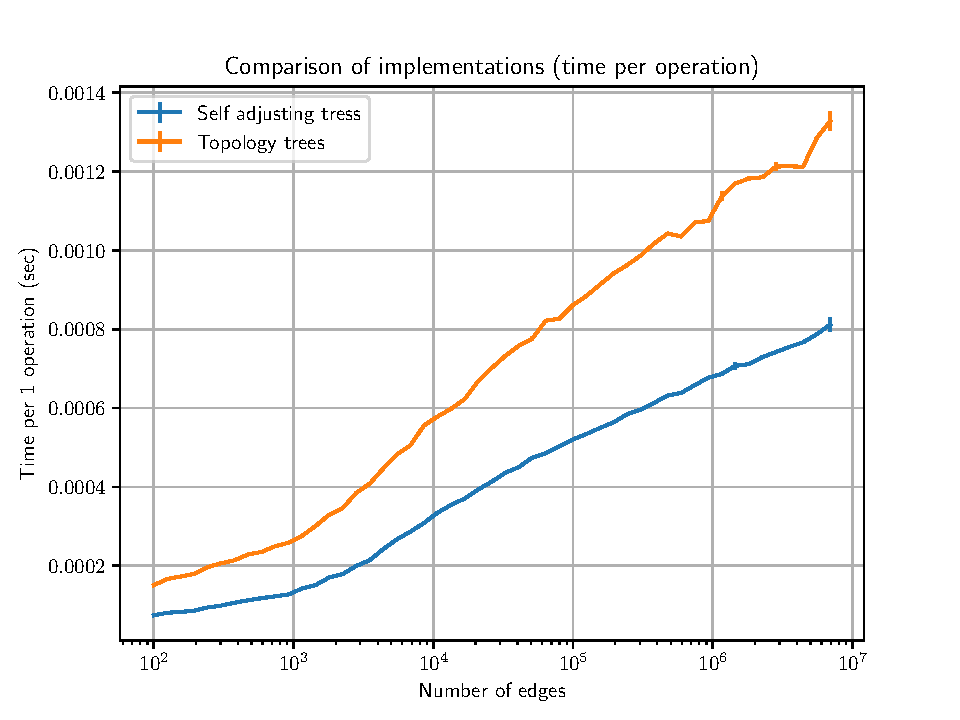
\includegraphics[width=10.4cm]{../charts/maximum_edge_weight_op.pdf}
	\end{figure}
\end{frame}

\begin{frame}{Maximum edge weight on path}
	\vskip -3mm
	\begin{figure}
	\centering
	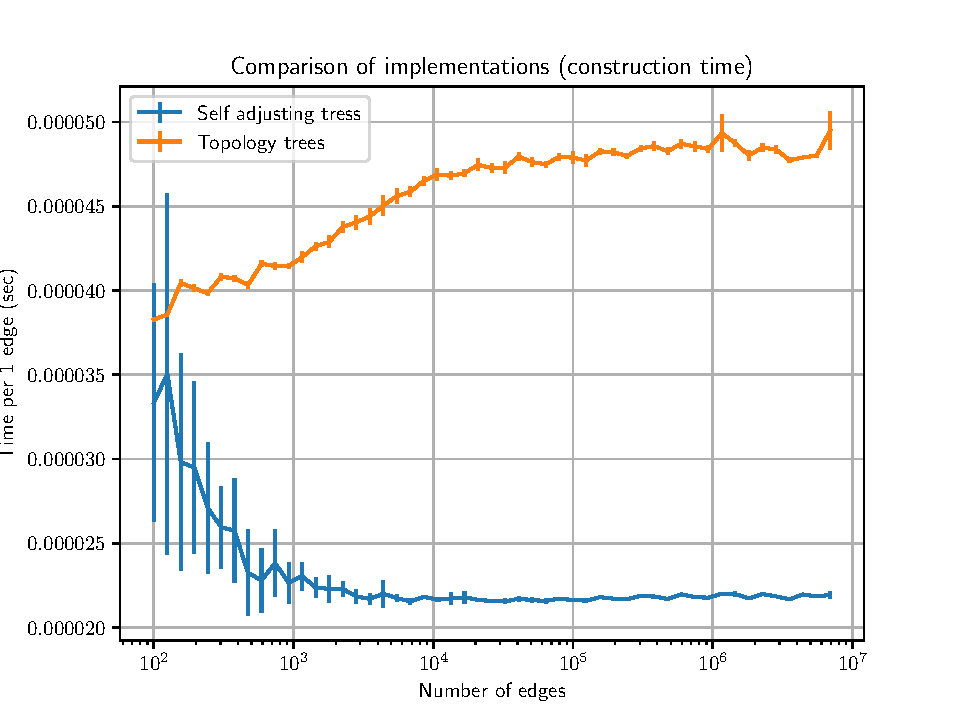
\includegraphics[width=10.4cm]{../charts/maximum_edge_weight_construction.pdf}
	\end{figure}
\end{frame}


\begin{frame}{Edge 2-connectivity}
	\vskip -3mm
	\begin{figure}
	\centering
	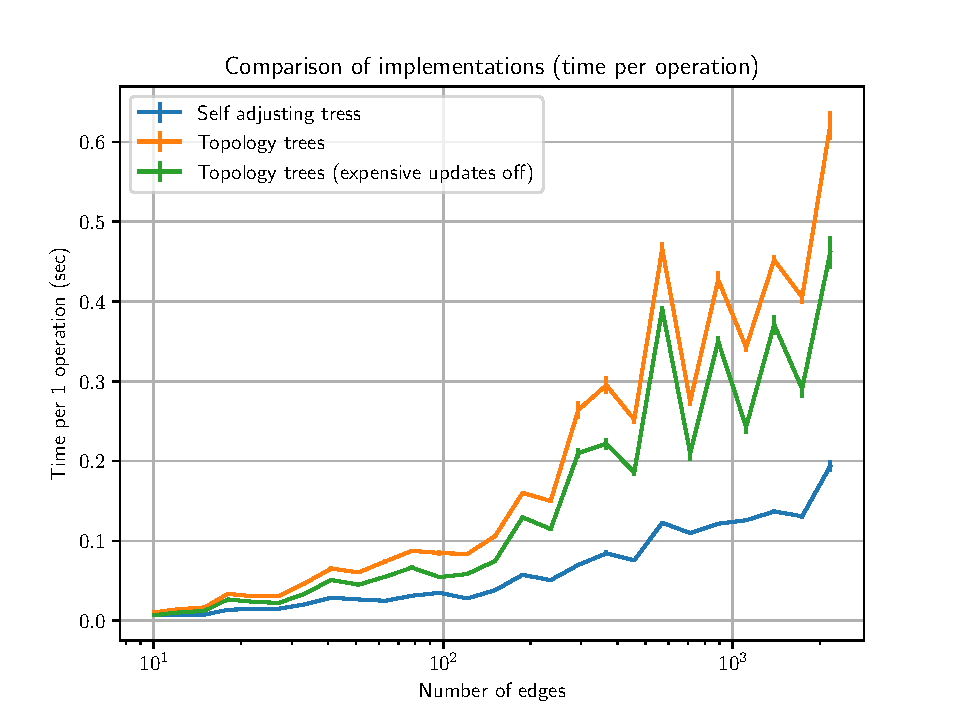
\includegraphics[width=10.4cm]{../charts/double_edge_connectivity_op.pdf}
	\end{figure}
\end{frame}

\begin{frame}{Edge 2-connectivity}
	\vskip -3mm
	\begin{figure}
	\centering
	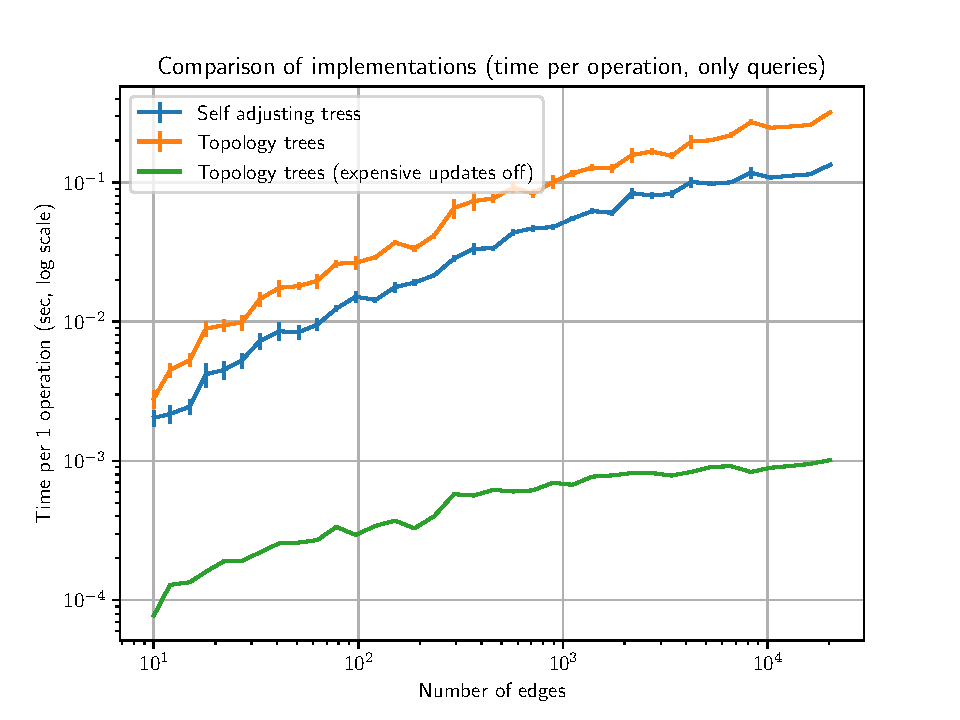
\includegraphics[width=10.4cm]{../charts/double_edge_connectivity_op_queries.pdf}
	\end{figure}
\end{frame}

%%%%%%%%%%%%%%%%%%%%%%%%%%%%%%%%%%%%%%%%%%%%%%%%%%%%%%%%%%%%%%%%%%%%%%%%%%%%%%%%

\section*{}
\begin{frame}{}

\centerline{I thank my supervisor Mgr. Vladan Majerech, Dr.}
\centerline{for this topic, advices and consultation}

\bigskip\bigskip

\centerline{Also I thank my opponent Mgr. Martin Mareš, Ph.D.}

\pause
\bigskip\hrule
\vfill
{\Large\centerline{Thanks for your attention}}
\vfill
\end{frame}

\end{document}
